\documentclass{article}

\title{\sc\LARGE CSCA67 Tutorial, Week 4\\
{\Large Oct. 5th-Oct. 9rd, 2015}}
\date{}
\author{\sc Compiled by {\em G. Singh Cadieux}\\[1ex]
\sc Adapted from\\
A. Bretscher, \href{http://www.utsc.utoronto.ca/~bretscher/a67/lectures/w4.pdf}{\em CSCA67 Week 4 Lecture Notes},\\
\href{http://www.intmath.com/counting-probability/6-probability-event.php}{\em Interactive Mathematics: Probability of an Event},\\
\href{http://www.intmath.com/counting-probability/singapore-toto.php}{\em Interactive Mathematics: Singapore TOTO} \&\\
\href{http://www.intmath.com/counting-probability/poker.php}{\em Interactive Mathematics: Probability and Poker}}

\usepackage{fullpage}
\usepackage{amsmath,amssymb}
\usepackage{color}
%\usepackage{multicol}
\usepackage{tikz}
\usepackage{hyperref}

\begin{document}
\maketitle

\section{\sc Review of last week's lecture}
\subsection*{\em More probability}

\subsection{\em Probability function}
A \textsc{probability function} is a function on a \textit{discrete} (containing a finite or countably infinite number of elements) sample space $\mathcal{S}$ that has domain $\mathcal{S}$ and satisfies
\begin{enumerate}
\item $0\leq P(A)\leq 1\;\text{for every event }A\subseteq\mathcal{S}$\\[1ex]
(That is, the probability of any event $A$ in \textsl{S} is between 0 and 1.)
\item $\sum\limits_{s\in \mathcal{S}}P(s)=P(\mathcal{S})=1,\;P(\emptyset)=0$\\[1ex]
(That is, the sum of the probabilities of every outcome in $\mathcal{S}$ is 1.\\
The probability of the entire sample space $\mathcal{S}$ - i.e., of any outcome in $\mathcal{S}$ occurring - is also 1.\\
The probability of the empty set - i.e., of no outcome in $\mathcal{S}$ occurring - is 0.)
\item $P(A_1\cup A_2\cup\ldots)=P(A_1)+P(A_2)+\ldots$ for \textit{disjoint} events $A_1,\,A_2,\ldots\subseteq \mathcal{S}$\\[1ex]
(That is, the probability of multiple, disjoint events $A_1,\,A_2,\ldots$ in $\mathcal{S}$ occurring is the sum of their individual probabilities.)
\end{enumerate}
\begin{description}
\item[\sc Disjoint:]\hfill\\
Two or more events $A_1,\,A_2,\ldots$ are disjoint if $A_1\cap A_2\cap\ldots=\emptyset$.\\[1ex]
(That is, if $i\neq j$, then $A_i$ and $A_j$ do not contain any of the same outcomes.)\\[1ex]
Represented as a Venn diagram:\\
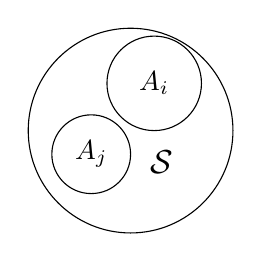
\begin{tikzpicture}
\draw (0,0) circle[radius=1.3];
\draw (0.3,0.6) circle[radius=0.6];
\draw (-.5,-0.3) circle[radius=0.5];
\node at (0.3,.6) {$A_i$};
\node at (-.5,-.3) {$A_j$};
\node at (0.4,-.4) {\large $\mathcal{S}$};
\end{tikzpicture}\\[1ex]
\textbf{eg.} for the experiment of throwing a standard die, events \{1, 3\}, \{4\}, and \{5, 6\} are disjoint
\end{description}

\subsection{\em Theorem: Complement rule}
If two events $E$ and $F$ are \textit{complementary}, then 
\begin{equation*}
P(E)=1-P(F)\Leftrightarrow P(F)=1-P(E)
\end{equation*}
\begin{description}
\item[\sc Complement:] The complement of any event $A$ is the event ``not A", i.e., the event that $A$ does not occur.\\
The event $A$ and its complement $\bar{A}$ are \textit{mutually exclusive} and \textit{exhaustive}; that is, $A$ and $\bar{A}$ cannot occur simultaneously (mutually exclusive), and all outcomes in $\mathcal{S}$ are represented in $A$ together with $\bar{A}$ (exhaustive).\\[1ex]
Represented as a Venn diagram:\\
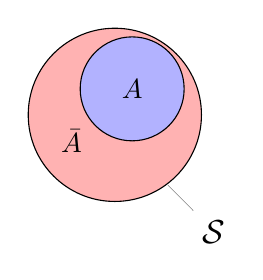
\begin{tikzpicture}[scale=1.1]
\draw[fill=red!30] (0,0) circle[radius=1];
\draw[fill=blue!30] (0.2,0.3) circle[radius=0.6];;
\node at (0.2,.3) {$A$};
\node at (-.5,-.3) {$\bar{A}$};
\node[pin=below right:{\large $\mathcal{S}$}] at (.5,-.7) {};
\end{tikzpicture}\\
\textbf{eg.} for the experiment of throwing a standard die, the complement of \{1, 2\} is \{3, 4, 5, 6\}
\end{description}

\section{\sc Probability problems}
\textsc{N.B. There are} several possible, equally valid ways to arrive at these answers, including different methods that may have been demonstrated in lecture.

\subsection{Singapore TOTO}
In the Singapore lottery game of TOTO, 6 (distinct) winning numbers plus one ``additional" winning number are drawn at random from the numbers 1 to 45. In the ordinary game, players choose 6 numbers/ticket in the hope of matching some or all of the winning numbers and becoming instant millionaires.

\subsubsection*{Prizes}
\begin{tabular}{|c|l|l|}\hline
Group&Prize Amount&Winning Numbers Matched\\\hline\hline
1&33\% of prize pool&6\\\hline
2&13\% of prize pool&5 + additional number\\\hline
3&13\% of prize pool&5\\\hline
4&13\% of prize pool&4 + additional number\\\hline
5&\$30 per winning combination&4\\\hline
6&\$20 per winning combination&3 + additional number\\\hline
\end{tabular}

\subsubsection*{Q: {\em What are the odds of being in Group 1?}}
Let us choose \textsl{S} = \{all combinations of 6 numbers from 1-45\}, so that our sample space represents all the possible combinations of 6 numbers from 1-45. Since the numbers are drawn at random, each outcome in the sample space is equally likely, so we can use the classical definition of probability:
\begin{equation*}
P(\{\text{Group 1}\})=\dfrac{|\{\text{Group 1}\}|}{|\textsl{S}|}
\end{equation*}
In this case, there is only 1 combination of 6 numbers we can choose that will cause us to be in Group 1: the 6 winning numbers. So
\begin{equation*}
P(\{\text{Group 1}\})=\dfrac{1\text{ winning combination}}{\binom{45}{6}\text{ possible combinations}}=\dfrac{1}{8\,145\,060}
\end{equation*}

\subsubsection*{Q: {\em What are the odds of being in Group 2?}}
The probability of being in Group 2 is the probability that we have chosen 5 winning numbers and 1 non-winning number, \textit{and} that the non-winning number is the additional number. We again use the classical definition of probability, and count the combinations of 6 numbers that contain 5 winning numbers and 1 non-winning number.
\begin{align*}
P(\{\text{Group 2}\})& =P(\{\text{5 winning numbers}\}\cap\{\text{1 additional number}\})\\
& =P(\{\text{5 winning numbers}\})\times P(\{\text{1 additional number}\})\\
& =\dfrac{|\{\text{5 winning numbers}\}|}{|\textsl{S}|}\times P(\{\text{1 additional number}\})
\end{align*}
There are $\binom{6}{5}$ ways in which we can choose 5 of the 6 winning numbers, and $\binom{39}{1}$ ways in which we can choose our sixth non-winning number from the 39 non-winning numbers. So by the product rule, there are $\binom{6}{5}\times\binom{39}{1}$ combinations of 5 winning numbers and 1 non-winning number.\\[1em]
The event of choosing the correct additional number from all possible additional numbers lies in a different sample space, which we will call \textsl{S'}. If \textsl{S'} = \{all possible additional numbers\}, then $|\textsl{S'}|=39$, since there are 39 possible additional numbers once the 6 winning numbers have been drawn.\\
Again, all outcomes in \textsl{S'} are equally likely, and there is only 1 way in which we can choose the correct additional number: our sixth, non-winning number must match the additional number. Thus,
\begin{equation*}
P(\{\text{Group 2}\})=\dfrac{\binom{6}{5}\times\binom{39}{1}}{\binom{45}{6}}\times \dfrac{1}{39}=\dfrac{6}{8\,145\,060}=\dfrac{1}{1\,355\,510}
\end{equation*}
Notice that the probability of being in Group 2 is 6 times the probability of being in Group 1.

\subsubsection*{Q: {\em What are the odds of being in Group 3?}}
The probability of being in Group 3 is the probability that we have chosen 5 winning numbers and 1 non-winning number, and that the non-winning number is \textit{not} the additional number.\\[1ex]
We calculated above that the probability of the former is $\dfrac{\binom{6}{5}\times\binom{39}{1}}{\binom{45}{6}}$.\\[1ex]
We also calculated that the probability of correctly choosing the additional number is $\frac{1}{39}$. By the complement rule, the probability of the complement, \textit{not} correctly choosing the additional number, is $1-\frac{1}{39}=\frac{38}{39}$. Thus,
\begin{align*}
P(\{\text{Group 3}\})& =P(\{\text{5 winning numbers}\}\cap\{\text{no additional number}\})\\
& =P(\{\text{5 winning numbers}\})\times P(\{\text{no additional number}\})\\
& =\dfrac{\binom{6}{5}\times\binom{39}{1}}{\binom{45}{6}}\times\dfrac{38}{39}\\
& =\dfrac{228}{8\,145\,060}=\dfrac{1}{35\,723.95}
\end{align*}

\subsubsection*{Q: {\em What are the odds of being in Group 4?}}
The probability of being in Group 4 is the probability that we have chosen 4 winning numbers and 2 non-winning numbers, \textit{and} that the non-winning number is the additional number.\\
There are $\binom{6}{4}$ ways in which we can choose 4 of the 6 winning numbers, and $\binom{39}{2}$ ways in which we can choose our 2 non-winning numbers from the 39 non-winning numbers. So by the product rule, there are $\binom{6}{4}\times\binom{39}{2}$ combinations of 4 winning numbers and 2 non-winning numbers.\\[1ex]
With regards to the additional number, there are 2 ways in which we can choose the correct additional number: either our first non-winning number matches the additional number, or our second non-winning number does. Thus,
\begin{align*}
P(\{\text{Group 4}\})& =P(\{\text{4 winning numbers}\}\cap\{\text{1 additional number}\})\\
& =P(\{\text{4 winning numbers}\})\times P(\{\text{1 additional number}\})\\
& =\dfrac{\binom{6}{4}\times\binom{39}{2}}{\binom{45}{6}}\times\dfrac{2}{39}\\
& =\dfrac{570}{8\,145\,060}=\dfrac{1}{14\,290}
\end{align*}

\subsubsection*{Q: {\em What are the odds of getting {\em any} prize?}}
The odds of getting \textit{any} prize are equivalent to the odds of belonging to \textit{any} group, that is, $P(\{\text{Group 1}\}\cup\{\text{Group 2}\}\cup\ldots\cup\{\text{Group 6}\})$. Since you cannot win more than one prize/belong to more than one group, these events are disjoint. Thus,
\begin{equation*}
P(\{\text{Group 1}\}\cup\{\text{Group 2}\}\cup\ldots\cup\{\text{Group 6}\})=P(\{\text{Group 1}\})+P(\{\text{Group 2}\})+\ldots+P(\{\text{Group 6}\})
\end{equation*}
If we were to calculate each of these probabilities, their sum would be $3.1197\times 10^{-3}$.

\subsubsection*{System entries}
In most lottery games, you can buy a ``system". Your chances of winning increase, but of course, you pay more as well.\\[1ex] 
For example, buying System 7 means you choose 7 numbers instead of the usual 6.\\
There are $\binom{7}{6}$ combinations of 6 numbers from 7, and so, System 7 gives you 7 times the chances of winning with an ordinary 6-number ticket.\\[1ex]
Suppose that you choose 1, 3, 5, 7, 9, 11, 13 as your 7 numbers. Then you will win if the winning numbers are any of these 7 combinations:
\begin{itemize}
\item 1, 3, 5, 7, 9, 11
\item 1, 3, 5, 7, 9, 13
\item 1, 3, 5, 7, 11, 13
\item 1, 3, 5, 9, 11, 13
\item 1, 3, 7, 9, 11, 13
\item 1, 5, 7, 9, 11, 13
\item 3, 5, 7, 9, 11, 13
\end{itemize}
In Singapore TOTO, you can buy up to System 12.

\subsubsection*{Q: {\em By how much do your chances of winning increase if you buy a System 12, relative to the chances of winning with an ordinary ticket?}}
Since there are $\binom{12}{6}=924$ combinations of 6 numbers from 12, there are 924 ways in which you can win, which is 924 times the single way in which you can win with only 6 numbers.

\subsection{Poker}
In the standard card game of poker, each player gets a hand of 5 cards and places a bet, hoping his hand is better than the other players' hands. The lower the probability of a hand occurring, the more valuable it is.\\[1ex]
The game is played with a pack containing 52 cards in 4 suits, consisting of:
\begin{itemize}
\item 13 hearts: \textcolor{red}{$\heartsuit$ 2 3 4 5 6 7 8 9 10 J Q K A}
\item 13 diamonds: \textcolor{red}{$\diamondsuit$ 2 3 4 5 6 7 8 9 10 J Q K A}
\item 13 clubs: $\clubsuit$ 2 3 4 5 6 7 8 9 10 J Q K A
\item 13 spades: $\spadesuit$ 2 3 4 5 6 7 8 9 10 J Q K A 
\end{itemize}

\subsubsection*{Ranking, frequency and probability of poker hands}
\begin{tabular}{|l|l|l|p{3in}|}\hline
\textsc{Hand}&\textsc{No. of Ways}&\textsc{Probability}&\textsc{Description}\\\hline\hline
Royal Flush&4&0.000002&Ten, J, Q, K, A of one suit.\\\hline
Straight Flush&36&0.000015&5 cards of one suit, in order.\newline
Example: 5, 6, 7, 8, 9, all spades.\\\hline
Four of a Kind&624&0.000240&4 cards of the same denominator.\newline Example: 4 kings and any other card.\\\hline
Full House&3744&0.001441&3 cards of one denominator and 2 cards of another.\newline Example: 3 aces and 2 kings.\\\hline
Flush&5108&0.001965&All 5 cards are from the same suit (excludes royal and straight flushes).\newline Example: 2, 4, 5, 9, J, all hearts.\\\hline
Straight&10\,200&0.003925&5 cards in order (excludes royal straight flushes).\newline Example: 3, 4, 5, 6, 7.\\\hline
Three of a Kind&54\,912&0.021129&3 cards of the same denominator.\newline Example: 3 aces, one J and one Q.\\\hline
Two Pairs&123\,552&0.047539&2 cards of one denominator and 2 cards of another.\newline Example: 3, 3, Q, Q, 5.\\\hline
One Pair&1\,098\,240&0.422569&2 cards of the same denominator.\newline Example: 10, 10, 4, 6, K.\\\hline
Nothing&1\,302\,540&0.501177&Example: 3, 6, 8, 9, K, collectively of at least two different suits.\\\hline
\end{tabular}

\subsubsection*{Q: {\em How do we know that the probability of being dealt a royal flush is 0.000002, as given above?}}
Let us choose \textsl{S} = \{all possible combinations of 5 cards\}. Since there are 52 cards in a deck, there are $\binom{52}{5}=2\,598\,960$ combinations of 5 cards.\\[1ex]
Only 4 of these combinations are royal flushes: (\textcolor{red}{$\heartsuit$ 10, J, Q, K, A}), (\textcolor{red}{$\diamondsuit$ 10, J, Q, K, A}), ($\clubsuit$ 10, J, Q, K, A), and ($\spadesuit$ 10, J, Q, K, A).\\[1ex]
Since all combinations of 5 cards are equally likely, we can use the classical definition of probability to determine that
\begin{equation*}
P(\{\text{royal flush}\})=\dfrac{|\{\text{royal flush}\}|}{|\textsl{S}|}=\dfrac{4}{2\,598\,960}\approx 0.000002
\end{equation*}

\subsubsection*{Q: {\em How do we know that the probability of being dealt a straight flush is 0.0.000015, as given above?}}
Within the same sample space as above, we need to determine the number of combinations of 5 cards that are straight flushes. For each suit, there are 10 straights: one that starts with a 2 (2, 3, 4, 5, 6), one that starts with a 3 (3, 4, 5, 6, 7), and so on, up to one that starts with a 10 (10, J, Q, K, A). Since there are 4 suits, there are $10\times 4=40$ possible straight flushes altogether. Thus,
\begin{equation*}
P(\{\text{straight flush}\})=\dfrac{|\{\text{straight flush}\}|}{|\textsl{S}|}=\dfrac{40}{2\,598\,960}\approx 0.000015
\end{equation*}
Note, however, that we should not strictly consider the royal flush, i.e. the straight flush starting with a 10, as a straight flush. If we exclude the royal flush, there are 9 straights for each suit, and $9\times 4=36$ in total. Then
\begin{equation*}
P(\{\text{straight flush}\})=\dfrac{|\{\text{straight flush}\}|}{|\textsl{S}|}=\dfrac{36}{2\,598\,960}\approx 0.000014
\end{equation*}

\subsubsection*{Q: {\em How do we know that the probability of being dealt a full house is 0.001441, as given above?}}
Within the same sample space as above, we need to determine the number of combinations of 5 cards that are full houses. We know that there are 13 denominators (2, 3, \ldots, A) and 4 cards of each denominator.\\[1ex]
If we select cards to form a full house, we must select 3 cards of 1 denominator and 2 cards of another. There are 13 ways to choose the denominator of the first 3 cards, and 12 ways to choose a different denominator for the next 2. Then, having chosen the denominator of each group, there are $\binom{4}{3}$ ways to choose 3 cards from 4 of the same denominator, and $\binom{4}{2}$ ways to choose 2 cards from 4 of the same denominator.\\[1ex]
Using the product rule, we determine that the number of ways in which we can choose a 5-card combination that is a full house is $13\times\binom{4}{3}\times 12\times\binom{4}{2}$, and so,
\begin{equation*}
P(\{\text{full house}\})=\dfrac{|\{\text{full house}\}|}{|\textsl{S}|}=\dfrac{13\times\binom{4}{3}\times 12\times\binom{4}{2}}{2\,598\,960}=\dfrac{3744}{2\,598\,960}\approx 0.001441
\end{equation*}

\section{\sc Additional practice problems}

{\bf Q: In Singapore TOTO, what are the odds of being in prize group 5?}\\[1em]
{\bf Q: In Singapore TOTO, what are the odds of being in prize group 6?}\\[1em]
On Monday, June 11th, 2001, the winning numbers for Singapore TOTO were 1, 10, 19, 23, 29, 45 with additional number 34. The next consecutive draw, on Thursday, June 14th, 2001, had the winning numbers 1, 10, 14, 19, 23, 34 with additional number 33.\\[1ex]
Thus, the five numbers 1, 10, 19, 23, 34 were repeated from the Monday draw. This is very rare and quite amazing.\\[1ex]
{\bf Q: What is the probability of this occurring?}\\[1em]
{\bf Q: For each hand of poker, as listed in (2.2), what is the probability of being dealt said hand?}

\end{document}